
\documentclass[letterpaper,hide notes,xcolor={table,svgnames},pdftex,10pt]{beamer}
\def\showexamples{t}


%\usepackage[svgnames]{xcolor}

%% Demo talk
%\documentclass[letterpaper,notes=show]{beamer}

\usecolortheme{crane}
\setbeamertemplate{navigation symbols}{}

\usetheme{MyPittsburgh}
%\usetheme{Frankfurt}

%\usepackage{tipa}

\usepackage{hyperref}
\usepackage{graphicx,xspace}
\usepackage[normalem]{ulem}
\usepackage{multicol}
\usepackage{amsmath,amssymb,amsthm,graphicx,xspace}
\newcommand\SF[1]{$\bigstar$\footnote{SF: #1}}

\usepackage[default]{sourcesanspro}
\usepackage[T1]{fontenc}

\newcounter{tmpnumSlide}
\newcounter{tmpnumNote}

% old question code
%\newcommand\question[1]{{$\bigstar$ \small \onlySlide{2}{#1}}}
% \newcommand\nquestion[1]{\ifdefined \presentationonly \textcircled{?} \fi \note{\par{\Large \textbf{?}} #1}}
% \newcommand\nanswer[1]{\note{\par{\Large \textbf{A}} #1}}


 \newcommand\mnote[1]{%
   \addtocounter{tmpnumSlide}{1}
   \ifdefined\showcues {~\tiny\fbox{\arabic{tmpnumSlide}}}\fi
   \note{\setlength{\parskip}{1ex}\addtocounter{tmpnumNote}{1}\textbf{\Large \arabic{tmpnumNote}:} {#1\par}}}

\newcommand\mmnote[1]{\note{\setlength{\parskip}{1ex}#1\par}}

%\newcommand\mnote[2][]{\ifdefined\handoutwithnotes {~\tiny\fbox{#1}}\fi
% \note{\setlength{\parskip}{1ex}\textbf{\Large #1:} #2\par}}

%\newcommand\mnote[2][]{{\tiny\fbox{#1}} \note{\setlength{\parskip}{1ex}\textbf{\Large #1:} #2\par}}

\newcommand\mquestion[2]{{~\color{red}\fbox{?}}\note{\setlength{\parskip}{1ex}\par{\Large \textbf{?}} #1} \note{\setlength{\parskip}{1ex}\par{\Large \textbf{A}} #2\par}\ifdefined \presentationonly \pause \fi}

\newcommand\blackboard[1]{%
\ifdefined   \showblackboard
  {#1}
  \else {\begin{center} \fbox{\colorbox{blue!30}{%
         \begin{minipage}{.95\linewidth}%
           \hspace{\stretch{1}} Some space intentionally left blank; done at the blackboard.%
         \end{minipage}}}\end{center}}%
         \fi%
}



%\newcommand\q{\tikz \node[thick,color=black,shape=circle]{?};}
%\newcommand\q{\ifdefined \presentationonly \textcircled{?} \fi}

\usepackage{listings}
\lstset{%
  keywordstyle=\bfseries,
  aboveskip=15pt,
  belowskip=15pt,
  captionpos=b,
  identifierstyle=\ttfamily,
  escapeinside={(*@}{@*)},
  stringstyle=\ttfamiliy,
  frame=lines,
  numbers=left, basicstyle=\scriptsize, numberstyle=\tiny, stepnumber=0, numbersep=2pt}

\usepackage{siunitx}
\newcommand\sius[1]{\num[group-separator = {,}]{#1}\si{\micro\second}}
\newcommand\sims[1]{\num[group-separator = {,}]{#1}\si{\milli\second}}
\newcommand\sins[1]{\num[group-separator = {,}]{#1}\si{\nano\second}}
\sisetup{group-separator = {,}, group-digits = true}

%% -------------------- tikz --------------------
\usepackage{tikz}
\usetikzlibrary{positioning}
\usetikzlibrary{arrows,backgrounds,automata,decorations.shapes,decorations.pathmorphing,decorations.markings,decorations.text}

\tikzstyle{place}=[circle,draw=blue!50,fill=blue!20,thick, inner sep=0pt,minimum size=6mm]
\tikzstyle{transition}=[rectangle,draw=black!50,fill=black!20,thick, inner sep=0pt,minimum size=4mm]

\tikzstyle{block}=[rectangle,draw=black, thick, inner sep=5pt]
\tikzstyle{bullet}=[circle,draw=black, fill=black, thin, inner sep=2pt]

\tikzstyle{pre}=[<-,shorten <=1pt,>=stealth',semithick]
\tikzstyle{post}=[->,shorten >=1pt,>=stealth',semithick]
\tikzstyle{bi}=[<->,shorten >=1pt,shorten <=1pt, >=stealth',semithick]

\tikzstyle{mut}=[-,>=stealth',semithick]

\tikzstyle{treereset}=[dashed,->, shorten >=1pt,>=stealth',thin]

\usepackage{ifmtarg}
\usepackage{xifthen}
\makeatletter
% new counter to now which frame it is within the sequence
\newcounter{multiframecounter}
% initialize buffer for previously used frame title
\gdef\lastframetitle{\textit{undefined}}
% new environment for a multi-frame
\newenvironment{multiframe}[1][]{%
\ifthenelse{\isempty{#1}}{%
% if no frame title was set via optional parameter,
% only increase sequence counter by 1
\addtocounter{multiframecounter}{1}%
}{%
% new frame title has been provided, thus
% reset sequence counter to 1 and buffer frame title for later use
\setcounter{multiframecounter}{1}%
\gdef\lastframetitle{#1}%
}%
% start conventional frame environment and
% automatically set frame title followed by sequence counter
\begin{frame}%
\frametitle{\lastframetitle~{\normalfont(\arabic{multiframecounter})}}%
}{%
\end{frame}%
}
\makeatother

\makeatletter
\newdimen\tu@tmpa%
\newdimen\ydiffl%
\newdimen\xdiffl%
\newcommand\ydiff[2]{%
    \coordinate (tmpnamea) at (#1);%
    \coordinate (tmpnameb) at (#2);%
    \pgfextracty{\tu@tmpa}{\pgfpointanchor{tmpnamea}{center}}%
    \pgfextracty{\ydiffl}{\pgfpointanchor{tmpnameb}{center}}%
    \advance\ydiffl by -\tu@tmpa%
}
\newcommand\xdiff[2]{%
    \coordinate (tmpnamea) at (#1);%
    \coordinate (tmpnameb) at (#2);%
    \pgfextractx{\tu@tmpa}{\pgfpointanchor{tmpnamea}{center}}%
    \pgfextractx{\xdiffl}{\pgfpointanchor{tmpnameb}{center}}%
    \advance\xdiffl by -\tu@tmpa%
}
\makeatother
\newcommand{\copyrightbox}[3][r]{%
\begin{tikzpicture}%
\node[inner sep=0pt,minimum size=2em](ciimage){#2};
\usefont{OT1}{phv}{n}{n}\fontsize{4}{4}\selectfont
\ydiff{ciimage.south}{ciimage.north}
\xdiff{ciimage.west}{ciimage.east}
\ifthenelse{\equal{#1}{r}}{%
\node[inner sep=0pt,right=1ex of ciimage.south east,anchor=north west,rotate=90]%
{\raggedleft\color{black!50}\parbox{\the\ydiffl}{\raggedright{}#3}};%
}{%
\ifthenelse{\equal{#1}{l}}{%
\node[inner sep=0pt,right=1ex of ciimage.south west,anchor=south west,rotate=90]%
{\raggedleft\color{black!50}\parbox{\the\ydiffl}{\raggedright{}#3}};%
}{%
\node[inner sep=0pt,below=1ex of ciimage.south west,anchor=north west]%
{\raggedleft\color{black!50}\parbox{\the\xdiffl}{\raggedright{}#3}};%
}
}
\end{tikzpicture}
}


%% --------------------

%\usepackage[excludeor]{everyhook}
%\PushPreHook{par}{\setbox0=\lastbox\llap{MUH}}\box0}

%\vspace*{\stretch{1}

%\setbox0=\lastbox \llap{\textbullet\enskip}\box0}

\setlength{\parskip}{\fill}

\newcommand\noskips{\setlength{\parskip}{1ex}}
\newcommand\doskips{\setlength{\parskip}{\fill}}

\newcommand\xx{\par\vspace*{\stretch{1}}\par}
\newcommand\xxs{\par\vspace*{2ex}\par}
\newcommand\tuple[1]{\langle #1 \rangle}
\newcommand\code[1]{{\sf \footnotesize #1}}
\newcommand\ex[1]{\uline{Example:} \ifdefined \presentationonly \pause \fi
  \ifdefined\showexamples#1\xspace\else{\uline{\hspace*{2cm}}}\fi}

\newcommand\ceil[1]{\lceil #1 \rceil}


\AtBeginSection[]
{
   \begin{frame}
       \frametitle{Outline}
       \tableofcontents[currentsection]
   \end{frame}
}



\pgfdeclarelayer{edgelayer}
\pgfdeclarelayer{nodelayer}
\pgfsetlayers{edgelayer,nodelayer,main}

\tikzstyle{none}=[inner sep=0pt]
\tikzstyle{rn}=[circle,fill=Red,draw=Black,line width=0.8 pt]
\tikzstyle{gn}=[circle,fill=Lime,draw=Black,line width=0.8 pt]
\tikzstyle{yn}=[circle,fill=Yellow,draw=Black,line width=0.8 pt]
\tikzstyle{empty}=[circle,fill=White,draw=Black]
\tikzstyle{bw} = [rectangle, draw, fill=blue!20, 
    text width=4em, text centered, rounded corners, minimum height=2em]
    
    \newcommand{\CcNote}[1]{% longname
	This work is licensed under the \textit{Creative Commons #1 3.0 License}.%
}
\newcommand{\CcImageBy}[1]{%
	\includegraphics[scale=#1]{creative_commons/cc_by_30.pdf}%
}
\newcommand{\CcImageSa}[1]{%
	\includegraphics[scale=#1]{creative_commons/cc_sa_30.pdf}%
}
\newcommand{\CcImageNc}[1]{%
	\includegraphics[scale=#1]{creative_commons/cc_nc_30.pdf}%
}
\newcommand{\CcGroupBySa}[2]{% zoom, gap
	\CcImageBy{#1}\hspace*{#2}\CcImageNc{#1}\hspace*{#2}\CcImageSa{#1}%
}
\newcommand{\CcLongnameByNcSa}{Attribution-NonCommercial-ShareAlike}

\newenvironment{changemargin}[1]{% 
  \begin{list}{}{% 
    \setlength{\topsep}{0pt}% 
    \setlength{\leftmargin}{#1}% 
    \setlength{\rightmargin}{1em}
    \setlength{\listparindent}{\parindent}% 
    \setlength{\itemindent}{\parindent}% 
    \setlength{\parsep}{\parskip}% 
  }% 
  \item[]}{\end{list}} 




\title{Lecture 19 --- Query Optimization}

\author{Jeff Zarnett \\ \small \texttt{jzarnett@uwaterloo.ca}}
\institute{Department of Electrical and Computer Engineering \\
  University of Waterloo}
\date{\today}


\begin{document}

\begin{frame}
  \titlepage

 \end{frame}


\begin{frame}
\frametitle{Query Optimization}

There are now some clear ways we can transform an input query to determine which of the equivalent representations will have the lowest cost of execution. 

It is fair to say that the query optimizer is likely to focus first on join relations since that is potentially the biggest area in which we can make some gains.

\end{frame}

\begin{frame}
\frametitle{Query Optimization}

Suppose our query involves a selection and a join. 

We want to select the employee number, salary, and address for an employee with an ID of 385. 

Suppose number and salary are in the employee table with 300 entries, and the address information is in another table with 12000 entries. 

We have a join query, and if we do this badly, we will compute the join of employees and addresses, producing some 300 results.

Then we need to do a selection and a projection on that intermediate relation.

If done efficiently, we will do the selection and projection first, meaning the join needs to match exactly one tuple of employees rather than all 300. 

\end{frame}

\begin{frame}
\frametitle{Query Optimization}
The query optimizer should systematically generate equivalent expressions. 

It is likely that the optimizer does not consider every possibility and will take some ``shortcuts'' rather than brute force this. 

One technique that helps on top of that is to re-use common subexpressions to reduce the amount of space used by representing the expressions during evaluation.


\end{frame}

\begin{frame}
\frametitle{Estimating Statistics}

In the previous example I used exact numbers, 300... 1... 12000... etc.,

But for the database server to get those it can either look them up, or it can guess about them. 

As mentioned earlier, sometimes certain numbers, like the number of tuples in a relation, are easily available by looking at metadata. 

If we want to know, however, how many employees have a salary between \$40~000 and \$50~000, the only way to be sure\footnote{Other than nuking it from orbit...} is to actually do the query.

And we don't want to do the query when estimating the cost...

\end{frame}


\begin{frame}
\frametitle{Guess we better... guess?}

If we cannot measure, then, well, we need to guess. Our guesses are, however, not wild, but instead educated. 

Estimates are based on assumptions, and those assumptions are very often wrong. 

That is okay. We do not need to be perfect. 

All we need is to be better than not optimizing.

And even if we pick the second or third or fifth best option, that is acceptable as long as we are close to the best option.


\end{frame}

\begin{frame}
\frametitle{Cost Centres}

There are five major areas where costs for actually performing a query accumulates. 

\begin{enumerate}
	\item \textbf{Disk I/O}
	\item \textbf{Disk Additional Storage}
	\item \textbf{Computation}
	\item \textbf{Memory}
	\item \textbf{Communication}
\end{enumerate}

We will generally proceed on the basis that disk I/O is the largest cost and outweighs everything else.

\end{frame}


\begin{frame}
\frametitle{Metadata}

Some items that might be in the metadata:

\begin{itemize}
	\item $n_{r}$: the number of tuples in a relation $r$ 
	\item $b_{r}$: The number of blocks containing a relation $r$ 
	\item $l_{r}$: the size in bytes of relation $r$
	\item $f_{r}$: the number of tuples of $r$ that fit into one block
	\item $V(A, r)$: the number of distinct values in $r$ of attribute $A$
	\item $h_{r, i}$: the height of an index $i$ defined on relation $r$
\end{itemize}

There can also be metadata about index information as well... which might make it metametadata?

\end{frame}



\begin{frame}
\frametitle{Maintaining Metadata}

The more often it is updated, the more effort is spent updating it. 

If every insertion or update or deletion resulted in an update, that may mean a nontrivial amount of time is spent updating this data. 

If we only do periodic updates, it likely means that the statistic data will be outdated when we go to retrieve it for use in a query optimization context. 

Perhaps some amount of balance is necessary...


\end{frame}

\begin{frame}
\frametitle{Histogram Data}

A database may also be interested in keeping some statistical information in a histogram. 

The values are divided into ranges and we have some idea of how many tuples are in those ranges. 

\begin{center}
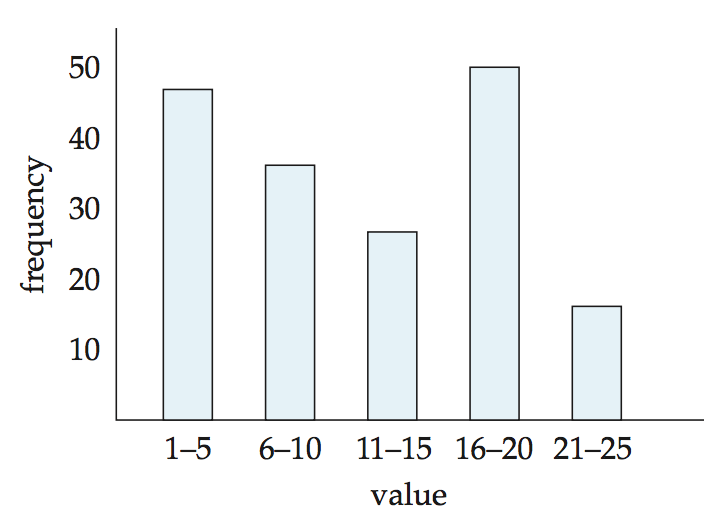
\includegraphics[width=0.4\textwidth]{images/histogram}
\end{center}

\end{frame}

\begin{frame}
\frametitle{Estimating Metadata}

The above numbers are exact values which we can know and, hopefully, trust. 

Although they could be slightly out of date depending on when exactly metadata updates are performed. 

The more exact values we have, the better our guesses. But things start to get interesting when we ask something that does not have a category.


\end{frame}

\begin{frame}
\frametitle{Estimating Sizes}

As in the previous discussion of costs, we expect select operations and join operations to be the important ones.

They are the ones we will do the most of (probably).

We will start with select operations.

\end{frame}

\begin{frame}
\frametitle{Single Equality Predicate}

The base case to consider is a single predicate in a selection with an equality condition (e.g., province = ``ON''). 

The estimate depends on what we know about the attribute $A$ referenced in the selection. 

If it is a key field, and therefore unique, we know the select will return 1 result. 

Unless, of course, it is not found and we will get zero results.

\end{frame}

\begin{frame}
\frametitle{Single Equality Predicate}

If values are evenly distributed, then we can expect that $n_{r}/V(A, r)$ tuples should be returned. 

If there are ten possible values and everything is approximately evenly distributed then a select is expected to produce 10\% of the tuples as its result. 

The uniform distribution may not be accurate, but if it is a reasonable approximation of the data, it is simple and fast. 

If a histogram is available, we can look in the range that contains that search value and guess based on the frequency count for that range instead.

\end{frame}


\begin{frame}
\frametitle{Single Comparison Predicate}

The next case is when we have a comparison like the salary greater than or equal to \$150~000. 

We can, using the known maximum and minimum values of this attribute, take a guess. 

If the requested value $v$ is less than the minimum, we expect no rows returned. 

If the requested value is greater than the max also zero. 

Otherwise, the formula to estimate, where $m$ is the minimum value and $M$ is the maximum value: $n_{r} \times \dfrac{v - m}{M - m}$

Of course, if a histogram is available, we would prefer to use that. 

\end{frame}

\begin{frame}
\frametitle{Complex Predicates}

For conjunction as well as disjunction, we will use a new symbol, $s$, which represents the selectivity of the a particular selection. 

How likely it is that a particular tuple matches a condition. 

The probability that a tuple satisfies $\theta_{i}$ is $s_{i}/n_{r}$.


\end{frame}

\begin{frame}
\frametitle{Complex Predicates}

For conjunctive selection, we want the probability that a certain tuple meets all of the criteria. 

So the formula to estimate is:

$n_{r} \times \dfrac{s_{1} \times s_{2}... \times s_{k}}{(n_{r})^{k}}$.


\end{frame}

\begin{frame}
\frametitle{Complex Predicates}

For disjunctive selection it is the probability of matching an one of those conditions. 

The calculation will be simplified by trying to compute 1 minus the probability it satisfies none of the conditions: 

$1 - (1 - \dfrac{s_{1}}{n_{r}}) \times (1 - \dfrac{s_{2}}{n_{r}}) \times ... \times (1 - \dfrac{s_{k}}{n_{r}})$

\end{frame}


\begin{frame}
\frametitle{Complex Predicates}

Negation is pretty simple.

If we have a predicate $\neg\theta$ then the number of tuples likely to meet that is the number of tuples in the relation subtract those that do match $\theta$.


\end{frame}

\begin{frame}
\frametitle{Estimating Join Size}

If we are computing a join where the relations have no attributes in common, then the ``join'' is really the cartesian product.

The number of tuples in the output will be the number of tuples in $r_{1}$ multiplied by the number of tuples in $r_{2}$. 

That's a lot.

\end{frame}

\begin{frame}
\frametitle{Estimating Join Size}

If the intersection of $r_{1}$ and $r_{2}$ is a key (unique value) for $r_{1}$ then we know that a tuple in $r_{2}$ can match with at most one in $r_{1}$.

So the maximum number of tuples that could occur is the number of tuples in $r_{2}$. 

If the intersection is also defined as a foreign key on $r_{2}$ then it is exactly the number of tuples in $r_{2}$. 

This also applies symmetrically (so you can swap $r_{1}$ and $r_{2}$ in the previous statements).


\end{frame}

\begin{frame}
\frametitle{Estimating Join Size: No Keys}

The difficult case occurs if the intersection of two relations is not a key in either of those two relations. 

In that case, looking at the attributes in the relation, which we will call $A$, then the number of tuples in the join relation are:

$\dfrac{n_{r_{2}}}{ V(A, r_{2})} $. 

Since we expect that they match with $r_{1}$ then we estimate that there will be:

$\dfrac{n_{r_{1}} \times n_{r_{2}}}{ V(A, r_{2})} $. 

\end{frame}

\begin{frame}
\frametitle{Estimating Join Size: No Keys}

The denominator here depends only on $r_{2}$...  

If you switched the positions of $r_{1}$ and $r_{2}$ we could get a different answer if $V(A, r_{1})$ is not identical to $V(A, r_{2})$. 

That is unusual but not impossible. 

If that is the case, we would choose the smaller of the two estimates.

\end{frame}

\begin{frame}
\frametitle{Projection}

Projection on an attribute $A$ will result in either $n_{r}$ tuples if duplicates are allowed, or $V(A, r)$ if they are not. 

The relational algebra definition does not permit duplicates, mind you.

\end{frame}

\begin{frame}
\frametitle{Aggregation}

Suppose we seek an aggregation on some attribute $B$ grouping by $A$.

 Imagine in an example that $B$ is salary and $A$ is job title. 
 
 Then there will be one tuple in the output for each distinct value of $A$.

\end{frame}

\begin{frame}
\frametitle{Set Operations}
If a set operation has both operands as the same relation, it can be rewritten as a compound predicate and that would give us our estimates. 

Those sorts of transformations are not especially difficult to imagine: 

$\sigma_{\theta_{1}}(r) \cup \sigma_{\theta_{2}}(r)$ is easily rewritten as $\sigma_{\theta_{1} \vee \theta{2}}(r)$. 


\end{frame}

\begin{frame}
\frametitle{Set Operations}

If the set operation is on different relations then we could actually estimate it directly. 

We will typically assume worst case scenario, so: 

(1) union will be the size of the two relations, 

(2) intersection will be the size of the smaller of the two relations, and 

(3) in set difference we will assume in $r_{1} - r_{2}$ that the result is the size of $r_{1}$ (i.e. no tuples removed). 

\end{frame}


\begin{frame}
\frametitle{Outer Join}

Outer joins are fairly simple. 

For a left outer join: $r_{1}$ {\tiny \textifsym{d|><|}} $r_{2}$ the estimated size is $r_{1} \bowtie r_{2}$ plus the size of $r_{1}$.

Right outer join $r{1} {\tiny \textifsym{|><|d}} r_{2}$ is estimated as $r_{1} \bowtie r_{2}$ plus the size of $r_{2}$. 

The full outer join {\tiny \textifsym{d|><|d}} is just the combined size of $r_{1}$ plus $r_{2}$.


\end{frame}

\begin{frame}
\frametitle{Distinct Values}

If we are interested in knowing how many distinct values of an attribute $A$ there are, we have a few shortcuts based on the query. 

The simplest possible case is if the query specifies that $A$ equals some value $a$ in which case there will be at most 1 distinct value of $A$. 

If the predicate is complex and there are several allowed values $a_{1}, a_{2}, a_{3}... a_{n}$ then we can be certain the maximum number of possible values of $A$ is $n$. 

The last easy case is if there is a comparison, in which case the estimate is $V(A,r) \times s$ where $s$ is the selectivity of the selection.


\end{frame}


\begin{frame}
\frametitle{Distinct Values}

Otherwise we will assume that the distribution of values of $A$ has no relation to the distribution of values in the selection predicate. 

The correct way to guess is through the use of probability theory. 

We could also do a quick estimate of the smallest value of $V(A, r)$ (the most restrictive selection condition). 

This same logic holds for estimating how many unique values will be returned in a join: the smallest condition will limit how many rows are in the relation.

\end{frame}


\begin{frame}
\frametitle{Advanced Query Optimization}

There are three more advanced techniques we will mention but not discuss deeply:

\begin{itemize}
	\item Top-K
	\item Update Ordering
	\item Multiquery Optimization
\end{itemize}


\end{frame}

\begin{frame}
\frametitle{Top-K}

Consider a query that asks you to find the top $k$ tuples based on some attribute, such as finding the top ten customers based on annual revenue. 

We could potentially save some work if we know that we need no further results are required.

For something like top customers by revenue, we would probably need to find all the tuples that match, aggregate them, and then sort by income...

\end{frame}


\begin{frame}
\frametitle{Update Ordering}

Update queries often have a bunch of conditions restricting them to one tuple. 

If that is the case, update optimization is not really an issue. 

But if the update affects a number of rows, then there is a possible problem called the \alert{Halloween problem}.

An updated tuple could be inserted into the relation ahead of where the scan is, meaning the tuple could be updated again incorrectly. 

\end{frame}

\begin{frame}
\frametitle{Update Ordering}

The problem can be solved in a few ways. 

One is to determine the tuples to be modified first before any updates take place. 

Another has to do with splitting up the updates to be done into batches so that we don't have to wait for the whole selection to be done.


\end{frame}


\begin{frame}
\frametitle{Multiquery Optimization}

The first way we can optimize multiple queries at once is to avoid repeating any operation that is used in more than one query. 

That is to say, if query 1 and query 2 both have some part in common, the result of that subquery should be reused rather than recomputed a second time. 

That would, of course, require that query 1 does not modify the data, which could cause a problem.

\end{frame}

\begin{frame}
\frametitle{Multiquery Optimization}

The second way to optimize when we have multiple queries is to do some things in parallel. 

Suppose query 3 scans over a particular relation $r$ looking for some attributes, and query 4 scans over the same relation $r$ looking for something different

We could note the tuples matching queries 3 and 4 in one single pass rather than having to scan it twice.



\end{frame}




\end{document}

